\chapter{if conversion \Author{C. Bruel}}
\inputprogress
\graphicspath{{img/}{if_conversion/img/}{part4/if_conversion/img/}}
	
\newcommand\cond{~?~}

TODO: talk about prof/feedback branch probabilities and beneficibility and objective function
TODO: write down algorithms

\section{Overview/Motivations}

We describe in this chapter an if-conversion framework in SSA, that allows to transform a regions of basic blocks into an a region were branches have been removed and instructions transformed into a conditional representation by the target architecture.
\subsection{Introduction}

In order to increase the instruction throughput, processors tend to increasing the number of instructions that can bin issued simultaneously. In order to fully exploit the parallelism made available by multiple issues processors \cite{Rau:2003:IP:1074100.1074489}, Instruction Level Parallelism techniques are implemented in the hardware, such as-out-of-order execution, or dynamic scheduling, branch prediction. However, a more economical trend delegates to the compiler the task to extract and organize ILP thu the envent of Explicitly scheduled architectures, such as EPIC (Explicitly Parallel Architectures), or VLIW (Very Large Instruction World).

Conditional branches introduce control dependencies between instructions. An instruction is control dependent on a preceding instruction if the first one determines the execution of the second one \cite{Kennedy:2001:OCM:502981}. They limit the scope of ILP optimizations, because they reduce the number of continuous instructions that are not data dependent and thus can be executed in parallel. By reducing the average size of a basic block, they act as a bottleneck for exposing parallelism.

If-conversion is the process of transforming a control flow region containing a several basic blocks into a single basic block of straight line of code. Thus removing control branches from this region \cite{Schlansker97achievinghigh}.

Removing branches improves performance in several ways: by removing the mis-prediction penalty, the instruction fetch throughput is increased and the instruction cache miss penalty reduced. Enlarging the size of the basic blocks allows the static scheduler to schedule earlier long latencies operations and to improve the ILP by merging multiple control paths into a single flows of execution. Many compiler optimizations are impacted by branches. Software Pipelining for example, can't efficiently schedule loops with conditional branches \cite{Warter:1992:EMS:144953.145796}.

Consider the following example, that represents the execution of a simple if-then-else statement on a 4-issue processor, with all instructions having a one cycle latency.

\begin{table}[ht]
\begin{minipage}[t]{.4\linewidth}
\centering
 \mbox{original code} \\
   \begin{tabular}{| l | l | l | l | }
    \hline
ALU1 & ALU2 & ALU3 & ALU4 \\
    \hline
$ p = cmp a $ & & & \\
$ p \cond br$ $l1$ & & & \\
$ x = g - 2 $ & $ y = g + 2 $ & & \\
$ br$ $ l2 $ & & & \\
$ l1: x = a + 1 $ & & & \\
$ l2: $ & & & \\
    \hline
    \end{tabular}
\end{minipage}
\begin{minipage}[t]{.4\linewidth}
\centering
\mbox{after speculative if-conversion} \\
    \begin{tabular}{| l | l | l | l | }
    \hline
ALU1 & ALU2 & ALU3 & ALU4 \\
    \hline
$ x_1 = g - 2 $ & $ x_2 = a + 1 $ & $y_1 = g + 2 $ & $ p = cmp a $ \\
$ p \cond x = x_1 : x_2 $ & $ p \cond y = y_1 : y_2 $ & & \\
    \hline
    \end{tabular}
\end{minipage}
\end{table}

The execution path is 3 cycles, regardless of the branch direction. Once if-converted, the instructions become independent from the test result, and can be executed in the cycle, reducing the execution path to 2 cycles.

We notice some important features with if-converted code. (we don't say predicated code on purpose, since predication is only a way to conditionalize code, as we will see further).

\begin{itemize}
\item variables have been renamed, 
\item a \textit{merge} pseudo operation have been introduced. It is necessary to reconstruct the original value of $x$ and $y$.
\item This \textit{merge} introdudcs a data dependency. if-conversion transforms control dependencies into data dependencies \cite{Allen:1983:CCD:567067.567085}. The first consequence is that all registers now live simultaneously, (live range), so the benefits of branch removing and better schedule balanced with increased live range and register pressure : If-conversion must rely on a powerfull decision model
\end{itemize}

\subsection{Architectural requirements}
In order to emit conditional code, the if-conversin algorithm expect the architecture to provide support for conditional execution of instructions, or to conditionaly commit the result of an instruction.
Basically, two kind of support can (co-)exist: predicated execution or speculive execution my mean of conditional moves.

Predication \ref{fig:pred} is an architectural features that allows an instruction to be executed conditionally my mean of a predicate (for pipelined architectured, the instruction is always executed, but the results is nullified). 

\begin{figure}
\begin{minipage}[t]{4cm}
\mbox{fully predicated:} \\
$ p \cond x = a + b $ \\
$ \overline{p} \cond x = 0 $ \\
\end{minipage}
\begin{minipage}[t]{4cm}
\mbox{partially predicated:} \\
$t = a + b $ \\
$p \cond x = t $ \\
$\overline{p} \cond x = 0 $ \\
\end{minipage}
\label{fig:pred}
\end{figure}

Speculation \ref{fig:spec} is a compiler technique that allows an instruction to be executed unconditionnally. If the condition is true, the result is commited. To be speculated, and instruction should not create have any other side effets. For instance a memory load should not be able to trap (cache misses can also be considered for performance). In order to bypass this limitation, architectures that relies on speculation for if-conversion useally provde a speculative load operantion that will not trap in case of invalid memory access. Those architectures must provide a instruction to commit the speculated value. select or conditional moves.

examples of conditional moves: cmov (Pentium Pro), select (ST 231 VLIW).

\begin{figure}
\begin{minipage}[t]{4cm}
\mbox{$cmov$ instruction:} \\
$t = a + b $ \\
$x = 0 $ \\
$x = cmoveq t $ \\
\end{minipage}
\begin{minipage}[t]{4cm}
\mbox{$select$ instruction:} \\
$t = a + b $ \\
$x = select p \cond t : 0 $ \\
\end{minipage}
\label{fig:spec}
\end{figure}

Another requirement: he condition code must be visible at the ISA level, to enable boolean optimisation of predicates.

\section{SSA if-conversion}

SSA provides an efficient intermediate representation in which all false data dependencies have been removed, thus removing the need for register renaming needed when merging two definitions into one. Each assignment target (def) is assigned a unique register name. Registers are re-materialized at join nodes using $\phi$ operations. A procedure is in minimal SSA form if the number of $\phi$ instructions at join nodes is as small as possible. SSA-form representation gives the properties that a variable is assigned only once, and their merging point is exposed info $\phi$ operations solves those problems. 

We noticed that the if-conversion requires a renaming process because each variable cannot be redefined when using a speculation model, and the insertion of a pseudo instruction to express the merging of the values comming from different paths. This looks like very much SSA, isn't it ?

\begin{figure}
\begin{minipage}[t]{4cm}
\mbox{original code in SSA:} \\
$ !cond br Label1 $ \\
$ x_1 = x_0 * 2 $ \\
$ y_1 = z_0 - 2 $ \\
$ br label2 $ \\
$ label1: $ \\
$ x_2 = x_0 + 1 $ \\
$ y_2 = y_0 - 1 $ \\
$ label2: $ \\
$ x = \phi (x_1,x_2) $ \\
\end{minipage} 
\begin{minipage}[t]{4cm} 
\mbox{after if-conversion} \\
$ x_1 = x * 2 $ \\
$ y_1 = z - 2 $ \\
$ x_2 = x + 1 $ \\
$ y_2 = y - 1 $ \\
$ x = \textit{merge}(x_1,x_2) $ \\
$ y = \textit{merge}(y_1,y_2) $ \\
\end{minipage}
\end{figure}

Starting from an sequence in SSA, the if-conversion algorithm for a simple region becomes amazingly straightforward: remove branches and replace $\phi$ operations. We must now resolve the problem of the representation of the conditionalized instruction while still in SSA mode after if-conversion. 

\subsection{A local and a global proble}

Locally, we notice then if-conversion require two problems to be solved.
\begin{itemize}
\item A renaming problem to avoid the multiple definitions of a different variables assignment merged into a single path. 
\item Minimize the number of instructions to be predicated. Only instruction that merge need to be conditionalized inside the predicate set that control the merge. Others can be safely speculated without the need of a special predicate reduction pass. Only the values that have ma merge point need to be conditionalized, other can be unconditionally executed.
\end {itemize}

Once the operations to be conditionalized have be isolated. The framework still need to answer two other questions: As a global problem the region to if-convert must be defined, using objective functions and branch probabilities to avoid moving to the hot path less frequently used instruction. Since if-conversion also transforms control flow dependencies into data flow dependencies, register pressure can become significantly high. Such decision function must take into account operations created by the process itself, such as predicate merging or new copies. 

During traditional if-conversion, for each basic block considered into the region, a predicate must be computed and assigned to the corresponding instructions. Finally predicated or speculative instructions must be emitted into the IR, and the SSA IR maintained. in \ref{fig:nest0}, instructions from BB1 are assigned with predicated $c$ and instructions from BB3 with predicated cq. \ref{fig:nest1} shows the code layyout after predicate assignements. In case of speculation mode, predicated instructions have to be converted into conditional moves, using temporaries to hold arithmentic values. Additionally, a new predicate will need 

\begin{figure}
\footnotesize
\begin{minipage}[b]{4cm}
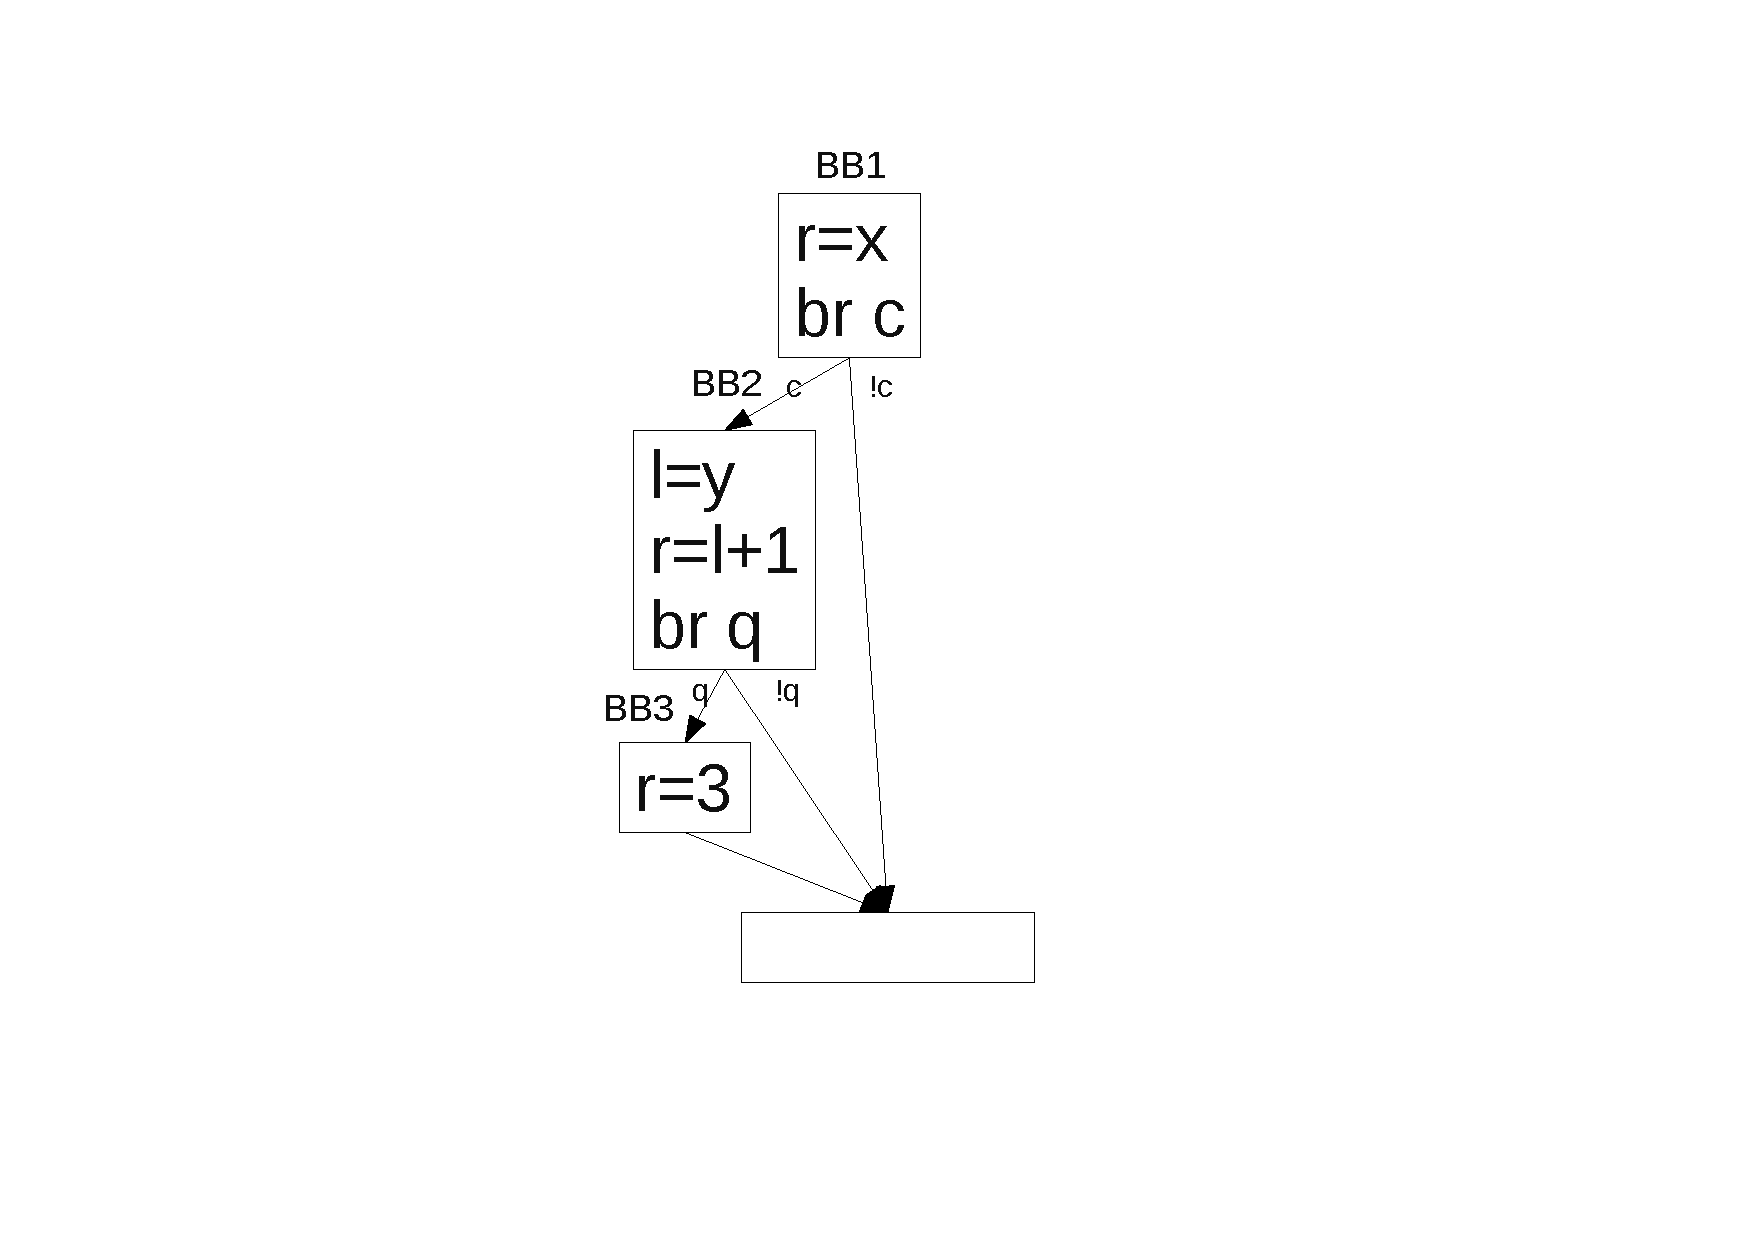
\includegraphics[scale=0.2]{nested_0.pdf}
\label{fig:nest0}
\end{minipage}
\begin{minipage}[b]{4cm}
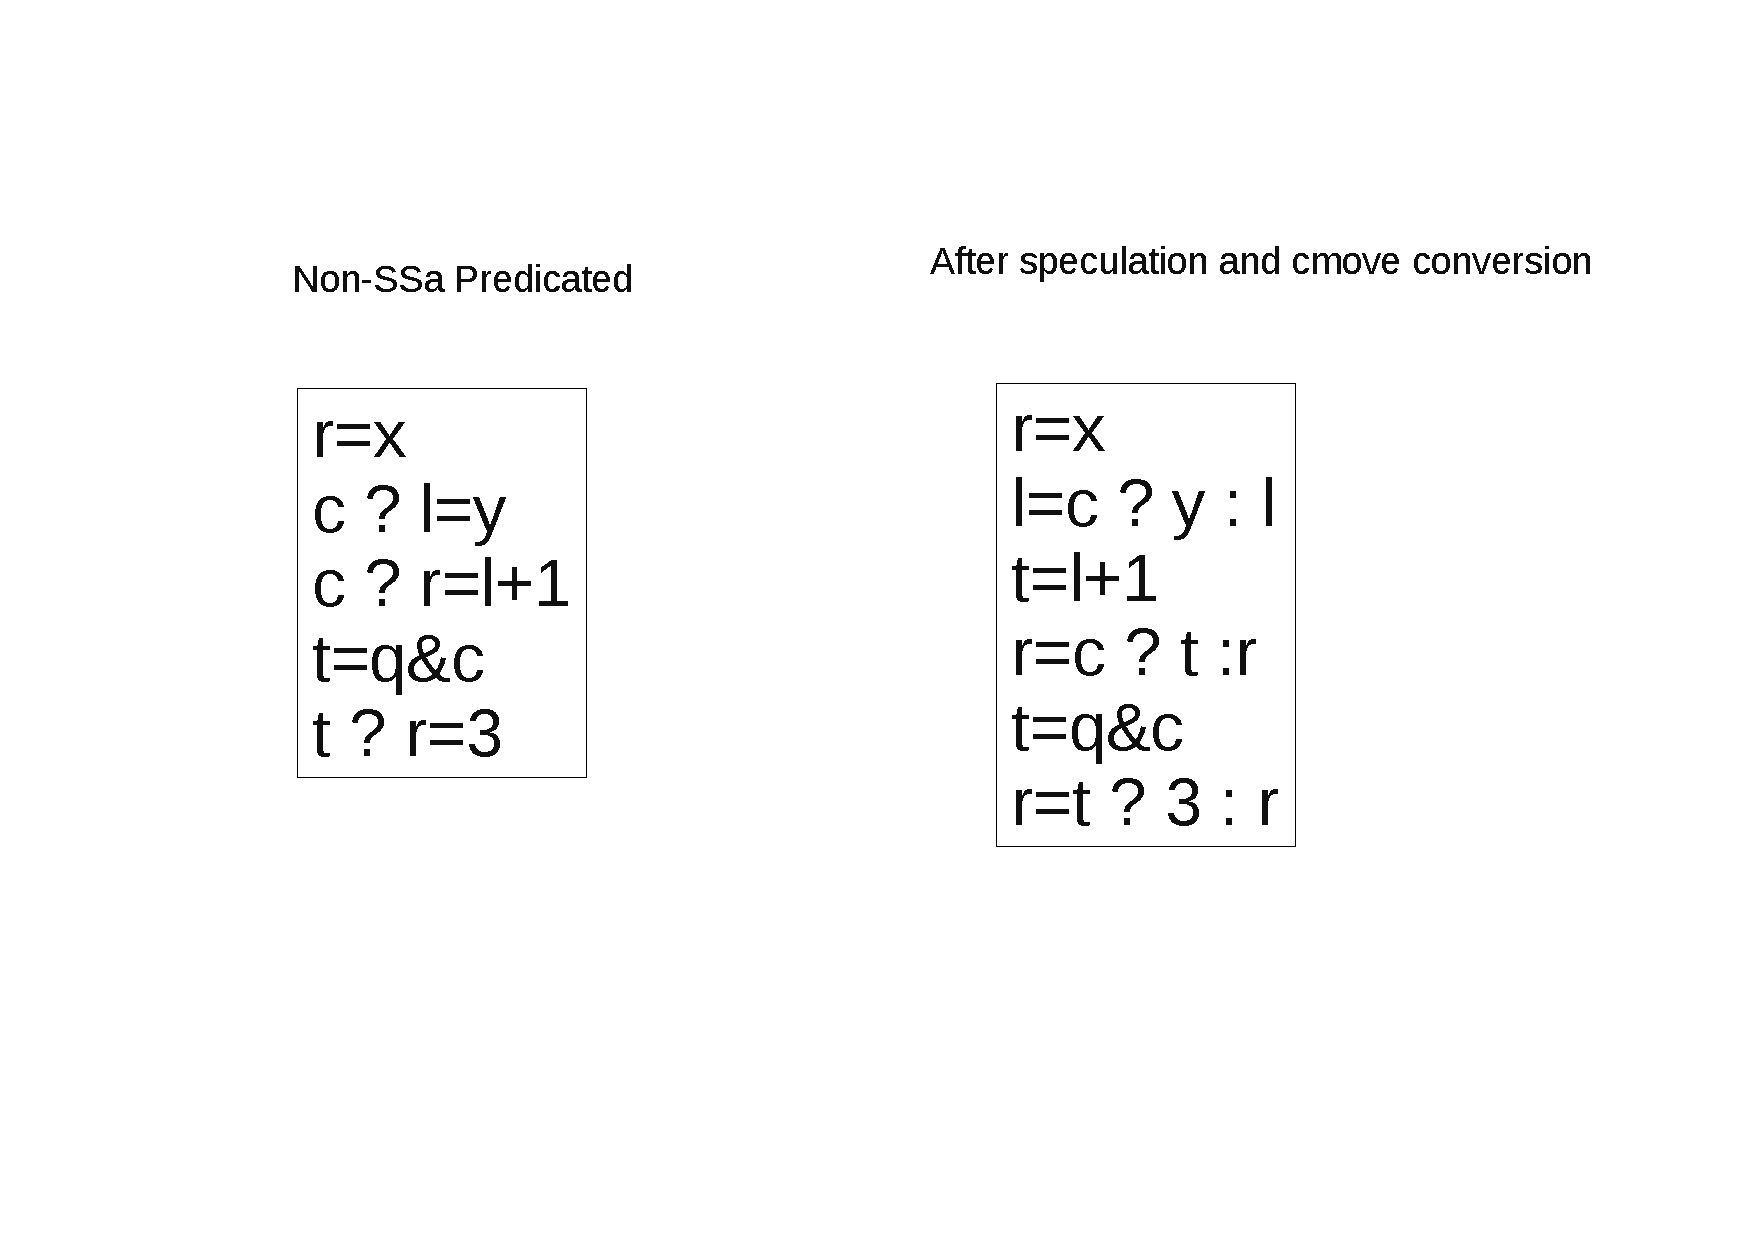
\includegraphics[scale=0.2]{nested_01.pdf}
\label{fig:nest1}
\end{minipage}
\caption{non-ssa code}
\end{figure}

In contrast, consider the equivalent SSA if-conversion 
Note that basically, Since a SSA $\phi$ express the merging point of $n$ definitions from $n$ predecessors, we can safely say the the definition points depends on their nearest condition under which they depend. Intuitively we already know that thanks to SSA the definition point is straightforward to find. Definitions not merging into a $\phi$ don't need to be conditionalized

This algorithm takes as input SSA form and produces either $\psi$-SSA if predicated instructions are available or pure SSA using select instructions to realized join points.

\subsection{SSA representation of conditional instructions}

In \ref{Stoutchinin:2001:ESS:563998.564022} $\psi$-SSA was described as a way to express a predicated form of SSA extension. Such representation is usually built from already predicated code, non SSA, originating from inlined assembly, peepholes, intrinsics functions or local transformations of control flow idioms. 

$\psi$-SSA expose the edge dependency from the basic block into which the definitionition of the $\phi$ argument is defined in the original CFG by a new data dependency. This dependency needs to be matemarialized into a $select$ or $\psi$ operation. Note that the $select$ operation is a real instruction that don't need to be replaced by the out-of-ssa process. If the target architecture doesn't provide such instruction to switch between speculated instruction, it can be emulated using two conditional moves. One advantage to generate $select$ instruction at this stage is that the program stays in full SSA form and make all the data dependencies explicit, and can be feed to all SSA optimizers. 

\begin{figure}
\begin{minipage}[t]{4cm}
\mbox{SSA:} \\
$ if (p) $ \\
$   x_1 = a+b $ \\
$ else $ \\
$   x_2 = 0 $ \\
$ x = \phi (x_1, x_2) $ \\
\end{minipage}
\begin{minipage}[t]{4cm}
\mbox{SSA-speculative form:} \\
$x_1 = a + b $ \\
$x_2 = 0 $ \\
$x = select p ? x_1, x_2$ \\
\end{minipage}
\begin{minipage}[t]{4cm}
\mbox{$\psi$-SSA form:} \\
$x_1 = a + b $ \\
$x_2 = 0 $\\
$x = \psi (p \cond x_1, \overline{p} x_2) $ \\
$y = \psi (p \cond x_1, \overline{p} x_2) $ \\
\end{minipage}
\end{figure}

Note that unlike $\phi$ arguments are executed simultaneously (they don't depend each other), $\psi$ arguments are executed sequentially and ordered from their definition predicate set. This propriety is necessary because if-conversion replaces the ``spacial'' dependency from the CFG by a ``temporal'' dependency from the straight line predicated code.

\subsection{SSA operations on basic blocks}

SSA if-convertion works itratively from inner regions to outer regions, using a set of transformations on conditional branches that we describe here.

\begin{figure}
\begin{minipage}[t]{5cm}
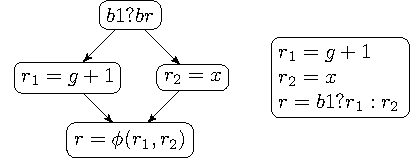
\includegraphics[scale=0.4]{phi_removal.pdf}
\caption{phi removal}
\label{fig:phi_rem}
\end{minipage}
\begin{minipage}[t]{5cm}
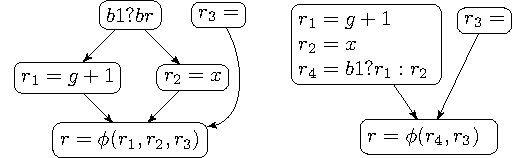
\includegraphics[scale=0.4]{phi_reduction.pdf}
\caption{phi reduction}
\label{fig:phi_red}
\end{minipage}
\begin{minipage}[t]{5cm}
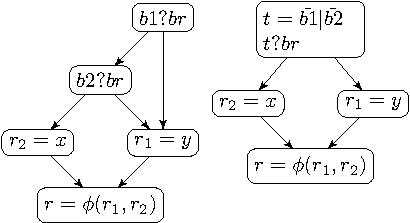
\includegraphics[scale=0.4]{phi_merge.pdf}
\caption{predicate merge}
\end{minipage}
\begin{minipage}[t]{5cm}
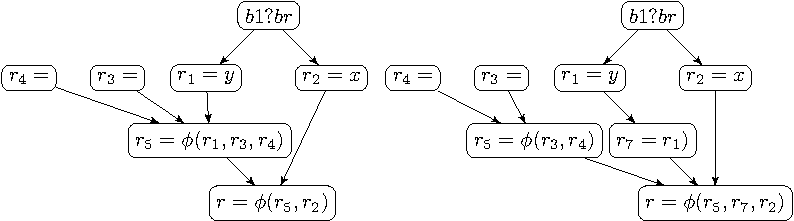
\includegraphics[scale=0.4]{phi_augmentation.pdf}
\caption{phi augmentation}
\label{fig:phi_aug}
\end{minipage}
\label{fig: phi_operations}
\end{figure}

The basic control structures that the analysis recognizes is the Single Exit region formed from the minimal set of blocks between a branch point and a merge point.  Those are minimal single entry single exit regions because at this point nested regions were already if-converted.

 We define this structure as the region between a conditional block and the first common immediate postdominator of the taken path block and the fall-thru block.

Note that each path can contain zero or more basic blocks with incoming edges.
As an optimization we allow two successive conditional blocks sharing one immediate post-dominator to be merged with logical operations after a normalization transformation. The normalization transformation ensures that conditional blocks sharing a same target can be merged by defining a wired $or$, or a wired $and$ share the same branch characteristics using branch reordering, test inversion or $de-morgan$ transformations.

\subsection{SSA maintenance}

Consider a conditional branch depending on a predicate $p$ and a region starting at $BBhead$. Let $BBp$ be the set of single exit basic blocks $(BBi,\dots,BB_n)$ that are on the taken path if $p$ is true and $BBq$ be the set of single exit basic blocks $(BBj,\dots,BB_m)$ that are executed if $p$ is false. The merge point of the if-converted region is at $BBjoin$. We distinct 4 types of basic SSA transformation that the framework uses and produces:
\subsubsection{$\phi$ removal} (figure \ref{fig:phi_rem})
The join node of the considered region has two predecessors and $\phi$ instructions are of the form $r=\phi(r_1,r_2)$. After speculation of the definitions of $r_1$ and $r_2$ the instruction can be rewritten as $r=\psi(p?r_1,\overline{p}?r_2)$.
\begin{proof} Once $BBp$ and $BBq$ have been promoted into $BBhead$, $BBjoin$ has for only predecessor $BBhead$ so it is not in its dominance frontier. The $\phi$ is not necessary and is removed.
\end{proof}
\subsubsection{$\phi$ reduction} (figure \ref{fig:phi_red})
 The join node of the considered region has $n$ predecessors that have $\phi$ instructions of the form $r=\phi(r_1,r_i,r_j,\dots,r_n)$. After merging, the $\phi$s are rewritten $t=\psi(p?r_i,\overline{p}?r_j)$ and a new $\phi$ $r=\phi(r_1,t,\dots,r_{n-1})$ is created with one operand less. The $\psi$ instruction is inserted after the speculated $r_i$ and $r_j$ definitions into $BBhead$.
\begin{proof} $BBjoin$ is still in the dominance frontier of $BBhead$, A $\phi$ must be redefined with the new definitions. The two corresponding $\phi$ edges from $BBq$ and $BBp$ can be replaced by the $BBhead$ edge.
The join block $E$ has $n$ predecessors with $n$ > 2, and $n$ blocks in its dominance frontier if it contains $\phi$s.
\end{proof}
\subsubsection{$\phi$ augmentation} (figure \ref{fig:phi_aug})
The objective is to remove incoming edges into the region. 
Consider a join node with $n$ predecessors among which $p$ is duplicated into $q$.  The join node of the considered region have $\phi$ instructions of the form $r=\phi(r_1,p,r_i,r_j,\dots,r_{n-1})$. The instruction is rewritten $t=select(p,r_i,r_j)$ and \mbox{$r=\phi(r_1,t,q,\dots,r_n)$}. 
\begin{proof}The duplicated blocks are new dominators of $BBjoin$ that define new $defs$. These blocks are now in the dominance frontier of $BBjoin$. SSA is maintained with new $\phi$ upgraded with the new reaching points.
Since the algorithm works the control flow in post order mode, the dominator tree doesn't change, and it's possible to maintain the SSA locally to the inner region. By recurence the if-converted region can be in turn be optimized out if it's head belongs to the dominance frontier of an outer region.
\end{proof}
Note that block duplication doesn't necessary implies more code size, since data flow dependencies are broken, noew oportunities for propagation or scalar optimisation arise. Here the local $t$ appears temporary, since $r2$ can be propagated into the $\phi$.

\subsection{SSA promotion}

To know the values that need to be conditionally written, we only need to look at the defining instructions of the $\phi$ instructions. By elimination, all temporaries that do not have a join point into the considered region and that don't have a side effect are unconditionally speculated during the SSA transformations processes. Instructions with a side effect will need to be guarded.

If-conversion converts control dependencies into data dependencies by computing a condition for the execution of each operation. Using our SSA framework, only operands from $\phi$ operations are considered to be conditional. This is an important advantage over traditional if-conversion algorithms that marks all instructions in a conditional basic block as dependent on the predicate. When considering dependency on a predicate we just walk from the $\phi$ uses to their definition points. All instructions are unconditionally speculated, but only those that are used in $\phi$ merge points that SSA exposes the conditional merging of values and generation of conditional moves.

Our algorithm is applied iteratively on a control flow in SSA form until no more reductions are possible. The quality of the SSA taken as input does not affect the correctness of the algorithm: if the control flow is in pruned SSA, i.e two paths $x->+z$ and $y->+z$ converge at node z, then a $\phi$ node is inserted at z only if z is alive in or after z. if which case x and y are promoted and no $select$ operation is generated. if the SSA is minimal, a $select$ instruction would be generated and removed by dead code. Inserting dead code from minimal SSA only introduces noise in the local scheduling heuristics because of the false data dependencies.

The basic idea behind the SSA transformations is to replace $\phi$ operations by predicated instructions merging into a $\psi$ or speculated instructions merging into a $select$ equivalent instructions, while maintaining the SSA properties. In figure \ref{fig:ssa} the conditional assignment uses a new temporary $r4$. Since the basic block containing the $\phi$ now has two incoming edges, a new $\phi$ is created to replace the former within the newly locally maintained SSA region.

The $select$ generation being done after instruction selection, the if-conversion framework can take opportunities for local optimizations such as conditional constant propagation like the $r2=2$ assignment in figure \ref{fig:ssa} if it can be absorbed by the $select$ instruction. Doing such optimizations locally enables the heuristics to be more precise in the formation of candidate if converted new regions.

\subsubsection{Partial redefinition}

A $\psi$ operation exposes new data dependencies, by expressing the merge of two definitions. Note that the order of the partial definition is important, so a definition partially redefines the preceding ones. We use this propriety to speculate the first definitions, so it becomes speculated instead of disjoint. This local optimisation allow to remove a predicate dependency but also creates a new partial dependency (predicates are not disjoint). Removing a predicate dependency is usually best because it allows to schedule the the expression earlier in the sequence

\begin{figure}
\footnotesize
\begin{minipage}{6cm}
$ p = test $ \\
$ p \cond x_1 = a + b $ \\
$ \overline{p} \cond x_2 = c $ \\
$ x = \psi(p \cond x_1, \overline{p} \cond x_2) $ \\
\caption{disjoint predicates}
\end{minipage}
\begin{minipage}{6cm}
$ x_1 = a + b $ \\
$ p = test $ \\
$ \overline{p} \cond x_2 = c $ \\
$ x = \psi(T \cond x_1, \overline{p} \cond x_2) $ \\
\caption{optimized order predicates}
\end{minipage}
\end{figure}

$T$ represents the $True$ predicate. This optimization is usefull to save one predicate register and to remove a data dependency between a predicate definition in its use. 
The $\psi$ definition is defined on the $T$ predicate set, therefore it is speculable, as shown here:

\subsubsection{$\psi$ speculation properties}

Since the algorithm process the regions from inner to outer, conditional operations will be in turn speculated or reconditionalized with a new condition. We define here $\psi$ operand promotion rules.

Consider the code \ref{fig:nested_psi}  containing a subregion already processed

Note the value produced in (4) is not defined for $p \& \overline{c}$ and $overline{p} \& \overline{c}$. Gladly all operations in defines $d_2 the \overline{c}$.

\subsubsection{$\psi$ predication properties}

If the instructions are not speculable, then they must be predicated:
The c condition must be merged with all conditions under which the phi operands are used. here d1 uses !p, so the psi can be rewritten as

We can see with this example that the decision to speculate or predicate can be done at the level of each joining definition, allowing a mix of them in the final program. The advantage to speculation over predication is a reduced dependency length. The disadvantage of speculation is that it increases register pressure untill the merge point, and put long latencies operation on the critical path.
 
\begin{figure}
\footnotesize
\begin{minipage}[b]{4cm}
$ if (c) $ \\
$ \{ $ \\
\hspace*{2mm}$ x_1 = a + b $ \\
\hspace*{2mm}$ \overline{p} \cond x_2 = c $ \\
\hspace*{2mm}$ x = \psi(T \cond x_1, \overline{p} \cond x_2) $ \\
\hspace*{2mm}$ d_1 = use (x) $ \\
$ \} $ \\
$ else $ \\
\hspace*{2mm}$ d_2 = 3 $ \\
$ d = \phi(d_1,d_2) $ \\
\caption{nested if}
\label{fig:nested_psi}
\end{minipage}
\begin{minipage}[b]{4cm}
$ x_1 = a + b $ \\
$ \overline{p} \cond x_2 = c $ \\
$ x = \psi(T \cond x_1, \overline{p} \cond x_2) $ \\
$ d_1 = use (x) $ \\
$ \overline{c} \cond d_2 = 3 $ \\
$ d = \psi(T \cond d_1, \overline{c} \cond d_2) $ \\
\caption{speculated nested if}
\label{fig:nested_psi_speculated}
\end{minipage}
\begin{minipage}[b]{4cm}
$ p_1 = \overline{p} \& {c} $ \\
$ c \cond x_1 = a + b $ \\
$ p_1 \cond x_2 = c $ \\
$ x = \psi(c \cond x_1, p_1 \cond x_2) $ \\
$ d_1 = use (x) $ \\
$ \overline{c} \cond d_2 = 3 $ \\
$ d = \psi(T \cond d_1, \overline{c} \cond d_2) $ \\
\caption{predicated nested if}
\label{fig:nested_psi_predicated}
\end{minipage}
\end{figure}

\subsubsection{Predicate merging}

During the regions formation, subregions containing a block that is reached from two conditions can be optimized by merging predicates. A new predicate is computed using a logical operation on both basic blocks' predicates after a normalization pass. Simple logical operations are usually caught as a peephole or during the instruction selection mechanism, but making it part of the if-conversion process allows it to handle more complex regions because our predicate merging algorithm is not limited to basic blocks that only define predicates, making instructions depending of predicates merge part of the generic SSA speculation framework. However, this transformation is very sensitive to biased branches since each conditional operation now depends on two predicates instead of one that cannot be scheduled together because of the computation of the logical operation making it more difficult to compensate for the branch removal. In order to avoid long sequences data dependencies and break schedule, we exclude from this promotion predicates that depend on long latency operations.
Because of new data dependencies introduced by the new computed predicate the performance contribution of this transformation mainly comes from the branch removal (two conditional branches and two direct branches are removed from a if-converted region whose predicates have been merged) rather than local ILP. Predicate promotion and merge is more effective in loop nest regions where more optimizations may extract ILP from it, for example modulo scheduling can extract ILP from such if-converted body by overlapping different iterations. 

\subsubsection{Block duplication}

Block duplication is used to remove side edges and to remove the constraints on control dependencies that enable the algorithm to find a set of basic blocks to if-convert. Unless applied carefully, we were afraid that block duplication could be the cause of code bloating without a performance counterpart. However experience has shown that when applied carefully it can be the source of very efficient if-conversion. Consider for example in the figure \ref{fig:bbdup}. Since we are if-converting from the inner most regions, the algorithm first considers the region {BB3,BB4,BB5,BB6,BB7}, and discards the edge coming from BB2 by duplicating BB6 into BB8. The $\phi$ becomes a move in the duplicated block with a renamed definition. The new $\phi$ operands are updated from the new edge. Note that in the implementation the block does not need to be created since it will be next promoted into BB3. We have two nested hammocks and the process can restart. The dependency that we removed in the control flow is now expressed as a data dependency between the two $select$ instructions.

The algorithm to perform SSA block duplication is decomposed into three steps: 
\begin{itemize}
\item Extract the $\phi$s 's def to be conditionalized from the duplicated block creating a $move$ instruction and a new reduced $\phi$ (or two $move$ instructions if the duplicated block had only two incoming edges).
\item Then the $\phi$s in the tail basic block are augmented with the new def created by the new repair instruction. If the $\phi$ was live-out after the tail block a move must be inserted to avoid propagating renaming outside of the region considered. 
\item The last step consists of renaming the new definitions to keep the region into SSA form.
\end{itemize}

\begin{figure}[th]
\begin{minipage}[b]{3cm}
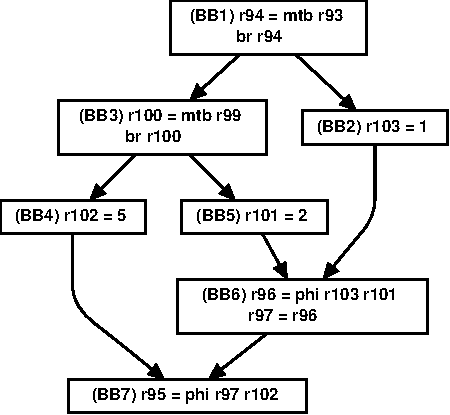
\includegraphics[scale=0.3]{g1.pdf}
\end{minipage}
\begin{minipage}[b]{3cm}
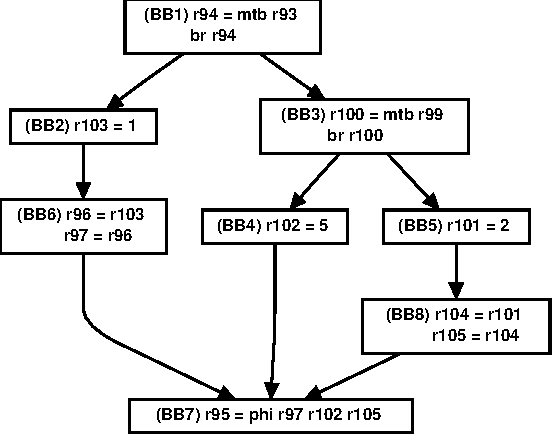
\includegraphics[scale=0.3]{g2.pdf}
\end{minipage}
\begin{minipage}[b]{3cm}
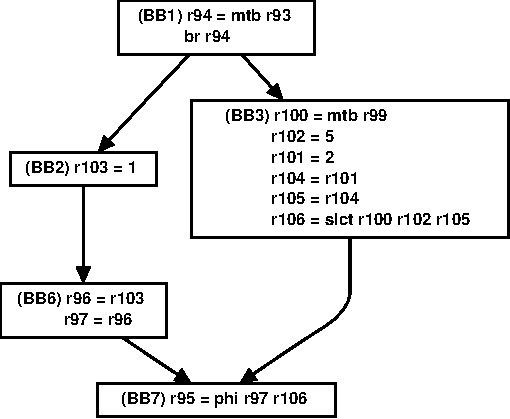
\includegraphics[scale=0.3]{g3.pdf}
\end{minipage}
\begin{minipage}[b]{3cm}
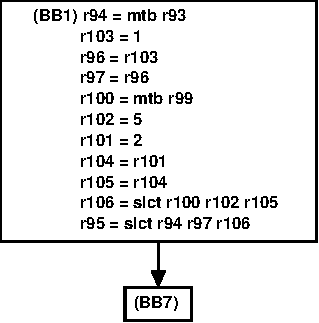
\includegraphics[scale=0.3]{g4.pdf}
\end{minipage}
\caption{Side entry removal using block duplication}
\label{fig:bbdup}
\end{figure}

\section{Global Framework}

\subsection{Profile support for if-conversion}

\subsection{Hyperblocks}

Traditional framework of if-conversion use Hperblocks as the basic predicated region formation. \cite{Mahlke:1992:ECS:144965.144998}. A hyperblock is a region of code with a single entry and multiple exits. Before the predicated code can be generated, the hyperblock excluding basic blocks that are not frequently executed, in order to combine only the common paths into the if-converted region, thus only optimizing the subset of the blocks within a give region (e.g a loop nest) are optimized. 

Several algorithmic or design choices impact the effectiveness of if-conversion. As an optimization, the region to if-convert, e.g hyperblock, must be just large enough to have the largest scope of scheduling framework, but in the same time it must not over-commit the machine resources (registers, CPUs). On the contrary, although if-conversion removes branches, I also add some overhead (new instructions to merge predicates, register pressure for speculative conditional, bigger dependence height because of the presence of new data dependencies on the predicates). The newly formed basic block doesn't have a higher schedule estimation than the one that would have been taken if the code was not if-converted.

For this reason, existing approaches of if-conversion are either limitted to a single conditional branch using peepholes style of pattern matching, intrinsic functions (conditional code is inlined by the compiler in the internal representation), or scoping larger but restricted regions such as loops hyperblocks. Such approaches require that the region is isolated from the rest of the control flow, , and more important requires a complicated estimation of the future if-converted region. So many factor impact this (predicate computation, register pressure, dependence height) that the objective function needs to be very conservative. Traditionally if-conversion cover the following steps:

\subsection{SSA Iterative if-conversion}

If you consider the control flow region from \ref{fig:hyper1} 

\begin{figure}[th]
\begin{minipage}[b]{3cm}
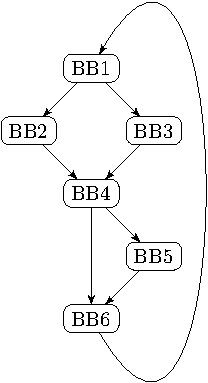
\includegraphics[scale=0.3]{hyper1.pdf}
\end{minipage}
\label{fig:hyper1}
\end{figure}

\begin{figure}[th]
\begin{minipage}[b]{3cm}
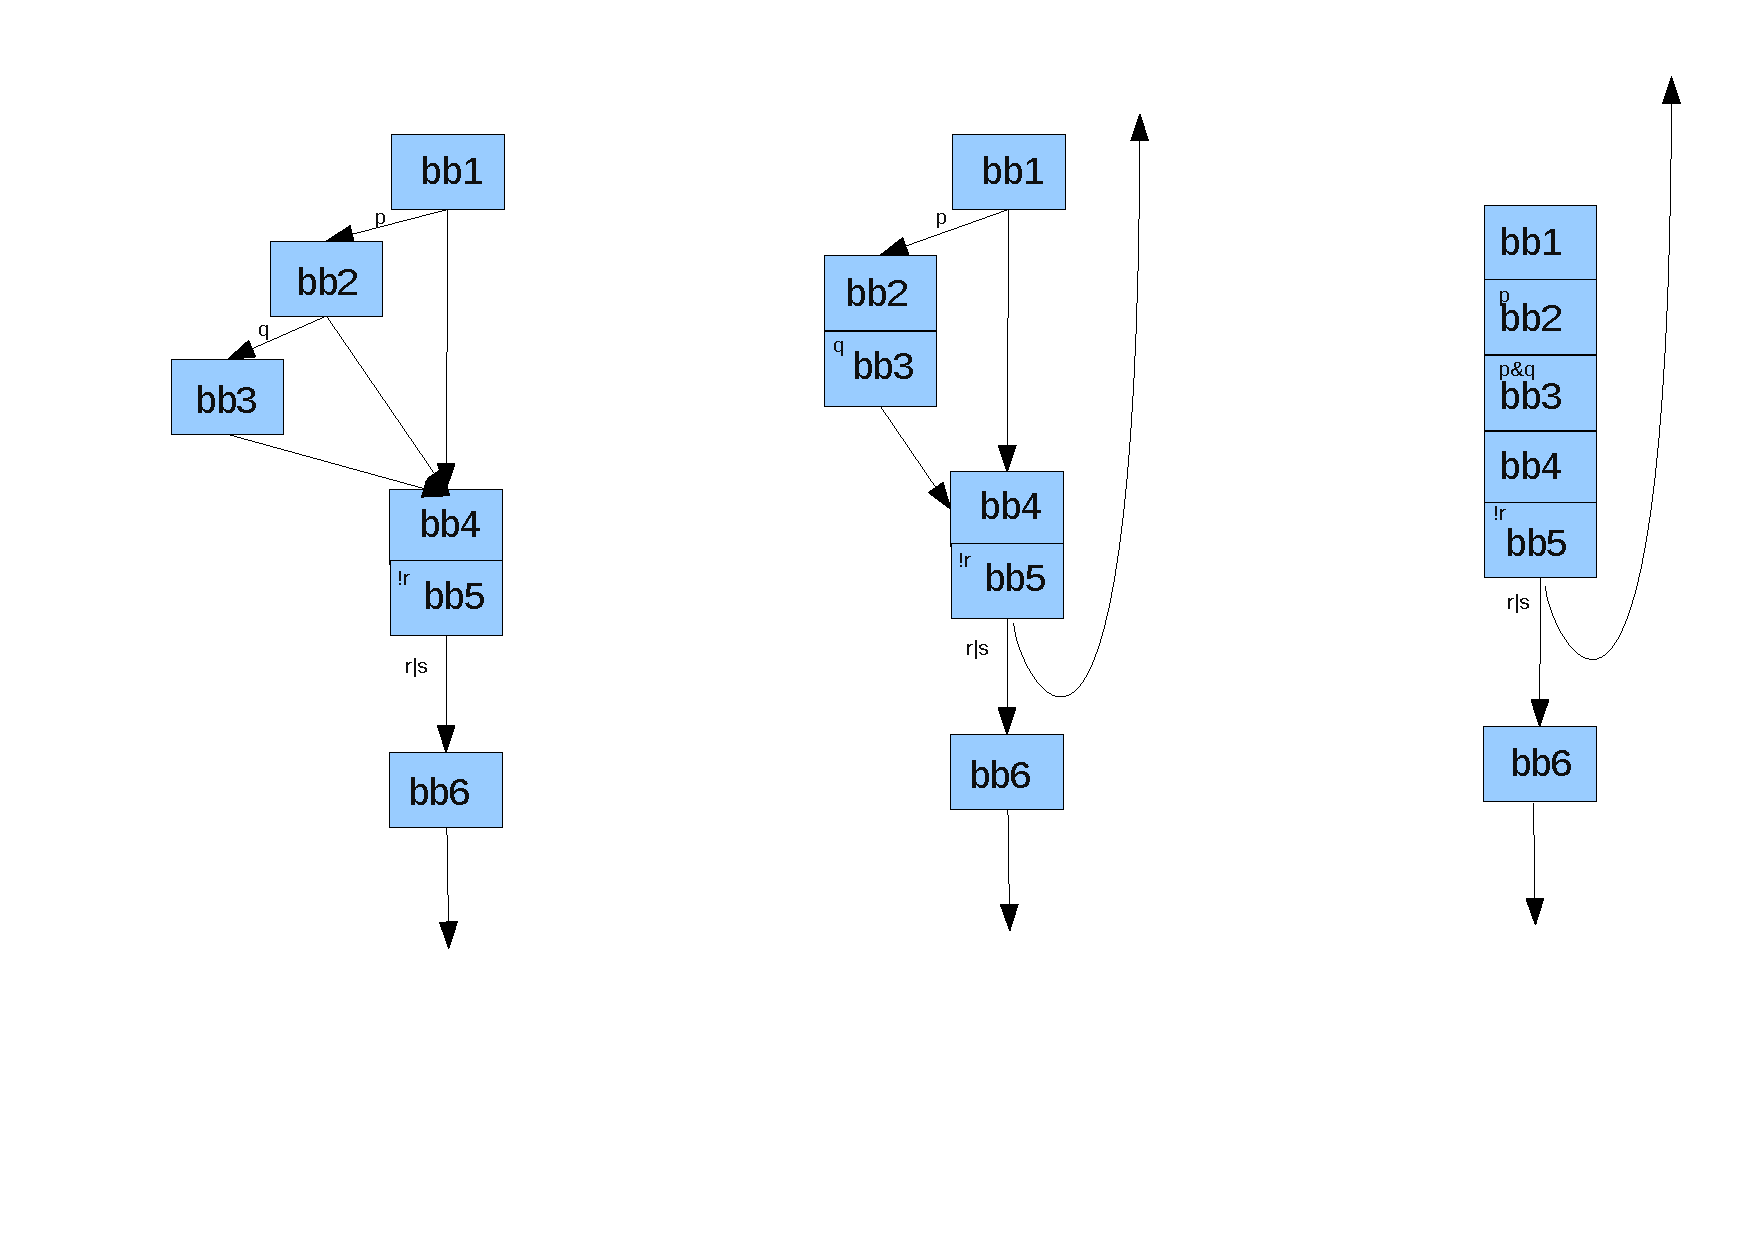
\includegraphics[scale=0.3]{hyper2.pdf}
\end{minipage}
\label{fig:hyper2}
\end{figure}

Conventional if-conversion algorithm should:

\begin{itemize}
\item Isolate the control flow region for which if-conversion is beneficial, using predictive heuristics. Using tail duplication to remove incoming edges. 
\item then for the whole region, Compute and assign a predicate to each basic block.
\item Convert the instructions into predicated ones using the predicate computed from the basic block, and merge the basic blocks.
\item Apply some predicate reduction mechanism to simplify predicate equations.
\item Finally emit the newly predicate computations and the predicated code. If the ISA is not fully predicated, an additional pass is needed to conditionalize them using conditional moves only.
\end{itemize}

In contrast, Using SSA iterative based if-conversion, \ref{fig:hyper1} all those steps become implicit, during the iterative SSA, Since the objective function has a finer granularity. On the case obove, the algorithm will proceed the conditioan absic blocs in postorder.
so first considering the region from {BB4,BB5,BB6} BB5 can be promoted to BB4, and the branch to BB6 becomes r\&q. This remove a branch from BB5 to BB6.
Then second, the region {BB2,BB3 is considered}. Then the region composed of {BB1,and BB2-3}. Finally the hyperblock was naturally formed.

All those operations make the if-conversion process a complex optimization, forcing designers to be extremely conservative, as the objective functions must contain variables not known at the start of the transformation. (such as the complexity of the predicate equations) since moving multiple control paths together can easily exceed processors resources (leading to excessive register pressure) or move infrequently used expensive instruction (memory loads) into the critical path. 

Set of transformations are applied iteratively and aggressively in postorder of the CFG
Start from first inner regions of basic blocks with a single conditional entry
Blocks reached on multiple conditions are detected (predicate merge)
Side entries removed using block duplication (less aggressive than tail duplication)
Decision to continue reconsidered for each region. ``The whole doesn't' exeed the sum of the parts''' or when hazardeous instructions

The process becomes a succession of local decisions, rather than a global decision. And can stop at anytime when the profitability of convertig a subnest is not established, or if a basic block has hazards. At this time, the decsion to stop to to proceed with tail duplication can be taken.

TODO: demonstrate
The SSA framework allows the decision functions to be accurate enough to avoid being too conservative and aggressively if-convert code, we will see in this chapter than an iterative bottom up process, on the SSA form can be more efficient, and more effective than the traditional top down techniques.

These operation are performed iterativelly on post order, consequently one of the propriety of the algorithms is that psi can be predicated. A Partial out of SSA can be iteratively performed on those regions by removing the $\phi$s and maintening a correct SSA internal representation. The algorithm takes SSA as input and produces SSA if a select instruction is available or $\psi$-SSA if predicated instructions are available. 

\subsubsection
Problem: phis into select was reazing join points
Transform select into the equivalent predicated instruction
Not SSA anymore: renaming problem: same variables defined 23 times on different predicatesd
wait after our of SSA do do a peephole transformation
Generate exenteded SSA for predication: psi

\section{Conclusion}
Easier to calculate beneficial optimisation locally and reconsider for each sub-region as the hyperblock grows, rather that globaly and reverse if-conversion
Only variables that join need to be conditionaliez, other can be speciulated if possible, reducing predicate dependencies

Speculated model: enter in strict SSA and produces strict SSA
Predicated model enter ins strict SSA and produces psi SSA.



